%!TEX root = ../main.tex

\section{Experimental setup}
\label{sec:setup}


\begin{figure}
    \centering
    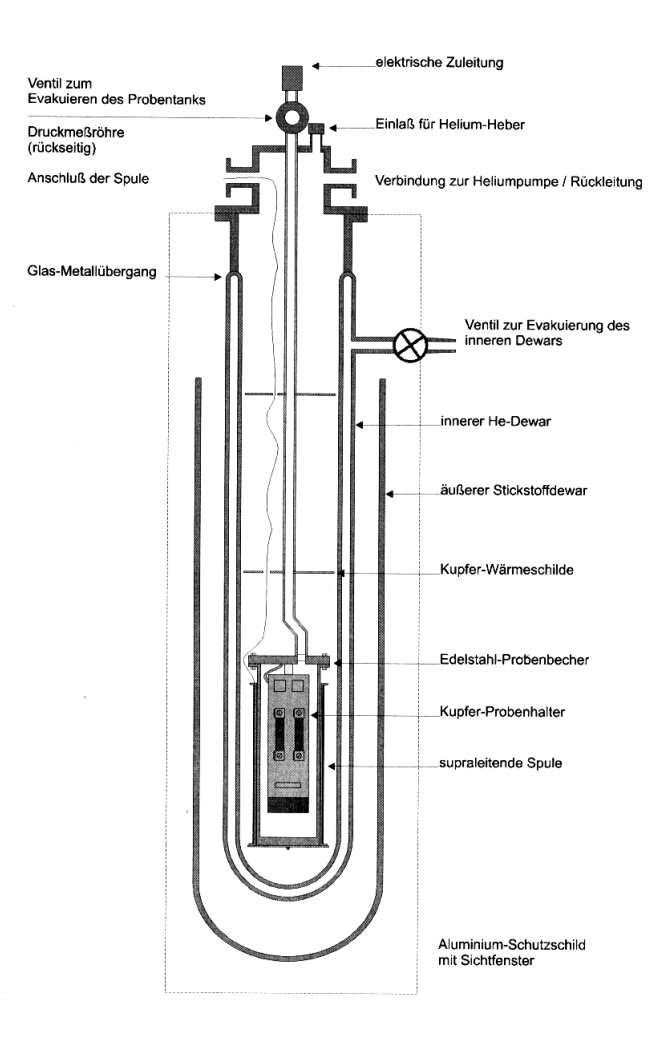
\includegraphics[width=0.8\textwidth]{./fig/kryo.png}
    \caption{Kryostat}
    \label{fig:kryo}
\end{figure}

The cryostat consists of two double-walled shells, so-called glass dewars (see figure $\autoref{fig:kryo}$). These allow thermal isolation from the room temperature. The outer glass dewar is filled with liquid nitrogen and cooled down to $\SI{80}{K}$. To reach lower temperatures, the inner glass dewar is cooled with liquid helium up to $\SI{5}{K}$. It also contains the sample cup with three samples: copper (metal), niobium (superconductor) and silicon (pure semiconductor). A superconducting coil is also attached to observe the behavior of niobium at the transition temperature with external magnetic field. 
A platinum and, from $\SI{30}{K}$, a carbon thermomenter are used to measure the 
temperature, at which the specific resistances are measured.
